% MDPI Systems submission-format manuscript.
% User-provided MDPI_Article_Template_2026-11-03_UserUploaded.zip.
% Definitions/mdpi.cls: June 23, 2026; journal option: systems; status: submit.
\documentclass[systems,article,submit,moreauthors]{Definitions/mdpi}
% The class provides: amsmath, amssymb, graphicx, booktabs, tabularx,
% multirow, microtype, enumitem, captions, hyperlinks, and geometry.
\usepackage{longtable}
\usepackage{ragged2e}
\setlength{\emergencystretch}{1.5em}
\setlength{\headheight}{20pt}
\newcommand{\NI}{\textit{not identified}}
\firstpage{1}
% MDPI submission placeholders; production assigns the real volume, issue and article number.
\pubvolume{1}
\issuenum{1}
\articlenumber{0}
\pubyear{2026}
\copyrightyear{2026}
\datereceived{}
\daterevised{}
\dateaccepted{}
\datepublished{}
\Title{Auditing Evidence Sufficiency for MSSP Portfolio Decisions: A Reproducible Protocol and Industrial Case}
\Author{Muhammad Emran $^{1,*}$ and Ghassan Malkawi $^{1}$}
\AuthorNames{Muhammad Emran and Ghassan Malkawi}
\address{$^{1}$ Faculty of Computer Information Science, Higher Colleges of Technology, Al Ain, United Arab Emirates; memran@hct.ac.ae (M.E.); gmalkawi@hct.ac.ae (G.M.)}
\corres{Correspondence: memran@hct.ac.ae}
\abstract{Portfolio plans can be internally traceable while remaining insufficient for particular managerial claims. We specify a claim-conditioned audit that distinguishes explicit source assertions from researcher-defined questions, admits records by version and intended scope, and separates parameter identification, target-specific bounds, and decision stability. A frozen prospective managed security service provider (MSSP) planning archive contains 51 detailed capabilities mapped exactly once into 25 consolidated packages. Its 49-service helper and narrative disagree with direct enumeration; the intended count definitions require reconciliation rather than an automatic accusation of operational error. Two packages bearing the same aggregate label give opposite results for a declared component predicate. The five-criterion priority matrix supports Firewall weak dominance over two alternatives under any nonnegative normalized numerical weights, but strictly positive illustrative weights make other areas the top scorer; the company's aggregation rule is undocumented. Under an explicit nonnegative additive financial interpretation, 12 family-year totals constrain 57 service-year unknowns, leaving 45 linear dimensions. Exact target bounds show that complete family sums may remain identified when individual service shares are not. Planned launch labels and exit criteria do not establish completed operations. A source-free executable specification and worked certificates are available, but independent human application, an authorized evidence-repair test and observed performance remain unverified. The contribution is a reproducible, single-case decision-specific evidence audit, not a new optimizer or field-effect estimate.}
\keyword{managed security services; source evidence; decision sufficiency; partial identification; robust preference; portfolio planning; cybersecurity governance}
\addhighlights{yes}
\renewcommand{\addhighlights}{%
\noindent\textbf{Contribution to systems science}\par
\begin{itemize}[leftmargin=1.4em,itemsep=1pt,topsep=2pt]
\item Admits evidence by claim origin, source version, unit, time and intended decision use across a coupled MSSP planning system.
\item Separates input identification, target-specific bounds and decision stability; unresolved inputs need not invalidate every decision.
\end{itemize}
\noindent\textbf{Main findings and implications}\par
\begin{itemize}[leftmargin=1.4em,itemsep=1pt,topsep=2pt]
\item All 51 capabilities map to 25 packages; identical package labels mask opposite component predicates and scorecard winners vary with weights.
\item Twelve family-year totals identify group sums but not arbitrary package shares; a public protocol documents exact bounds and evidence requests.
\end{itemize}}
% Override the MDPI submission-template's default left-sidebar copyright line.
% An author-review copy has not been submitted or licensed under CC BY.
\renewcommand{\cright}{\raggedright\textbf{Copyright:} \copyright{} 2026 by the authors. Manuscript prepared for review; not submitted or published. Reuse license not yet assigned.}
\begin{document}
% DRAFT REVIEW DISPLAY ONLY: the MDPI class generates a fictitious DOI from
% volume/issue/article-number placeholders. Suppress that display in this
% pre-submission author manuscript. MDPI production will assign real metadata.
\fancyhead[L]{\fontsize{8}{8}\selectfont Author manuscript prepared for \emph{Systems} (not yet submitted)}
\fancyfoot[R]{\fontsize{8}{8}\selectfont DOI not assigned}
\fancypagestyle{plain}{%
  \fancyhf{}%
  \fancyhead[L]{\fontsize{8}{8}\selectfont Author manuscript prepared for \emph{Systems}}%
  \fancyfoot[L]{\fontsize{8}{8}\selectfont Manuscript for author review; not published}%
  \fancyfoot[R]{\fontsize{8}{8}\selectfont DOI not assigned}%
}

\section{Introduction}
Managed security service providers (MSSPs) increasingly package operational, governance, identity, data-security, and human-risk capabilities into recurring service portfolios. This creates a familiar portfolio question---which offerings to launch, when, and under which assumptions---and an accompanying evidence question: \emph{what can the planning record establish for a particular requested decision?}

Service-portfolio research provides structures for representing and evaluating portfolios \cite{Kohlborn2009,Comerio2015}; heterogeneous service-repository integration addresses correspondences and representational conflicts \cite{BatiniComerio2016}; new-service-development research separates service identification, modelling, implementation, and commercialization \cite{LinHsieh2011,MenorRoth2008}; and robust portfolio methods already address incomplete costs and interdependencies \cite{Liesio2008,Tavana2019}. MSSP economics and information-security outsourcing are established topics \cite{GuptaZhdanov2012,Wu2017}. Likewise, sensitivity to criterion weights is established in multi-criteria decision analysis (MCDA) \cite{Maliene2018}. We therefore do not propose a new optimizer, maturity index, or MCDA method.

The narrower problem is that commercial planning artifacts operate at different levels of granularity. A detailed capability may be collapsed into a package; a package may inherit a single status and launch year; five focus areas may receive ordinal score vectors without an explicit aggregation rule; financial forecasts may be available only by family; and key performance indicator (KPI) rows may contain planned targets rather than observations. If these layers are treated as interchangeable, a roadmap can appear quantitatively precise while an individual service-level claim remains unresolved. Conversely, an unknown component quantity need not alter a decision that is robust across all admissible values.

From a systems perspective, the object of study is the \emph{coupled planning-decision architecture}, not the accuracy of an isolated spreadsheet. Its documented layers link named capabilities to packages, package labels to staged availability, criterion scores to portfolio priorities, and family-level resources and revenue to proposed commercial choices. A cross-layer inference is admissible only when its source unit, timing, intended use and evidentiary role survive that transition. This is an analysis of \emph{documented decision dependencies}; it neither models actual operational feedback loops nor measures organizational or cybersecurity performance.

We examine this problem in a prospective MSSP transformation case. The parent archive contains 25 entries: 23 material entries and two export-error text records. Two pairs of material entries are byte-identical copies, leaving 21 distinct material payloads. Nine selected source files form the quantitative and cross-format audit, while one distinct weekly reflection provides a contextual approval-status check. The source-admission and exclusion summary appears in Appendix~\ref{app:source}; the exact-path audit ledger remains restricted to authorized investigators. These artifacts document successive planning drafts, not repeated company deployments. Draft-2 and Draft-3 do not represent observed before/after performance; they are successive planning versions. Draft-3 is the primary analytical source and contains a 51-capability catalogue, a 25-package consolidation, five focus areas, a three-year roadmap, resource/KPI models, and a five-family financial scenario.

The study asks four research questions:
\begin{enumerate}[leftmargin=1.5em]
\item \textbf{RQ1 -- Claim and source alignment.} Which claims were actually recorded, which were introduced analytically, and what component information survives capability-to-package aggregation?
\item \textbf{RQ2 -- Decision-rule stability and stage scope.} Which focus comparisons are invariant under a clearly labelled numerical rule class, which change across admissible diagnostic weights, and what launch-scope distinctions remain unresolved?
\item \textbf{RQ3 -- Financial target identification.} Under a declared nonnegative additive interpretation, which financial targets are identified or bounded by family totals, and what does not follow about service delay effects?
\item \textbf{RQ4 -- Operational evidence.} Which planned conditions are source facts, and which claims about achieved release, service-level agreement (SLA) or key performance indicator (KPI) performance require later observed evidence?
\end{enumerate}

The contributions are (i) a specified evidence-admission and claim-origin protocol with structured outputs, (ii) an industrial demonstration of both resolved and unresolved cross-layer questions through verifiable witnesses, and (iii) exact source-free diagnostics for weight-dependent preferences and financial target bounds, with explicit requests for further evidence. Repository reconciliation, claims--arguments--evidence, robust portfolio methods and partial identification are prior art, not claimed inventions. This paper does not measure an improvement over existing audit practice. Crucially, a missing parameter is not by itself a reason to halt every decision: identification is checked against the \emph{requested target or action}, not merely every entry of a model.

\section{Related Work and Positioning}
\subsection{Service portfolios, incomplete information, and decision rules}
Kohlborn et al. conceptualize service portfolio management through goals, tasks, governance, methods, and enablers \cite{Kohlborn2009}; Comerio et al. formalize a repository-oriented service portfolio and design metrics \cite{Comerio2015}. More directly, Batini and Comerio address integration of heterogeneous service repositories by identifying correspondences among service representations \cite{BatiniComerio2016}. Our 51-to-25 check therefore cannot claim to invent cross-repository reconciliation: it asks which \emph{decision-specific} facts remain recoverable after source-authored consolidation. Lin and Hsieh distinguish service identification from later implementation and commercialization activities \cite{LinHsieh2011}. These frameworks motivate a key distinction in the present case: being listed in a portfolio is not equivalent to having the evidence required to claim operational release.

Incomplete information is not new to portfolio decision support. Liesi\"o et al. develop robust portfolio models with incomplete costs and project interdependencies \cite{Liesio2008}, while Tavana et al. apply hybrid portfolio selection in a cybersecurity-industry context \cite{Tavana2019}. MCDA rankings are also known to depend on criterion weights and their sensitivity \cite{Maliene2018}. Our scorecard analysis is therefore a case-specific identifiability diagnostic, not a new weighting method.


\subsection{How the present study extends prior work}
Table~\ref{tab:priorwork} positions the contribution as an upstream complement rather than a replacement for established portfolio, MSSP, and quality-assurance methods. The common thread is that prior methods need a decision object---a service, project, cost, score, contract, or measure---whose meaning is sufficiently specified. The present study tests that precondition directly in a multi-artifact industrial roadmap.

\begin{table}[H]
\centering\footnotesize
\caption{Closest methodological strands: established work and the distinct bounded operation tested here. No comparative performance is inferred.}
\label{tab:priorwork}
\begin{tabularx}{\linewidth}{>{\raggedright\arraybackslash}p{3.35cm} X X}
\toprule
Established strand & What is already known & Claim-specific operation in this case\\
\midrule
Service portfolio and service development \cite{Kohlborn2009,Comerio2015,BatiniComerio2016,LinHsieh2011,MenorRoth2008} & Portfolio governance, repository reconciliation and the distinction between service design and execution. & Exact mapping is an integrity control; a package label is tested against a component predicate rather than assumed to prove release.\\
Robust and multi-criteria portfolio decision support \cite{Liesio2008,Tavana2019,Maliene2018} & Incomplete parameters can be handled within defined admissible sets; ordinal ranking depends on the interpretation of weights. & Distinguishes identified targets, stable pairwise comparisons and ambiguous global leaders; weights are analytical examples only.\\
MSSP economics and spreadsheet quality \cite{GuptaZhdanov2012,Wu2017,Cezar2017,Powell2008,Poon2024} & Outsourcing and financial incentives are complex; spreadsheet quality-assurance issues are established. & Checks source-to-target financial identification rather than treating draft financial totals as service-level earnings.\\
Cyber decisions, assurance evidence and source scope \cite{Dawson2026,GSNv3,SACM2023,Mohamad2021,MohamadEvidence2024,Viger2026} & Decision uncertainty, evidence linkage, missing records and defeaters are established subjects. & Adds typed source/unit admission, explicit question origin and a conditional witness; no superiority over assurance review is claimed.\\
Partial identification \cite{Manski2005} & Under incomplete restrictions, identification is a property of a target and its admissible set. & Provides exact target-bound and decision-sufficiency certificates under stated finite additive assumptions.\\
\bottomrule
\end{tabularx}
\end{table}

These comparisons identify scientific ancestry, \emph{not} empirical superiority to prior methods. In particular, the presence-only contrast in Table~\ref{tab:contrast} is deliberately weaker than a full assurance-case review, OSCAL assessment, or robust portfolio model. Taken together, these studies define the foundation on which the present case builds. Service-portfolio and new-service-development work explains what must be managed; robust and multi-criteria portfolio models explain how choices can be optimized under uncertainty; MSSP research explains economic and sourcing incentives; spreadsheet and security-measurement research explains why evidence quality matters. Our narrower contribution is a \emph{claim-specific sufficiency} test: establish whether a requested target or comparison is determined, bounded, robust to incomplete inputs, or still reliant on a missing authorized rule. Robust optimization can legitimately proceed with nonunique parameters when its decision is shown to remain valid over the admitted set.

\subsection{Assurance arguments and identification sets: the closest methodological precedents}
Security assurance cases explicitly relate claims, assumptions, arguments, and supporting evidence; the Goal Structuring Notation and OMG Structured Assurance Case Metamodel already formalize this family of reasoning \cite{GSNv3,SACM2023}. A systematic review by Mohamad et al. examines security assurance cases and their practical validation limitations \cite{Mohamad2021}. Subsequent interviews in six safety-critical organizations document the challenges of identifying and managing security evidence \cite{MohamadEvidence2024}; an assurance-case study of the Large Hadron Collider demonstrates that a structured argument can expose previously undocumented defeaters \cite{Viger2026}. These are materially close precedents: neither missing-evidence recognition nor structured rebuttal is novel here. Thus the present paper does \emph{not} claim to invent evidence sufficiency, provenance, or claim--evidence linkage. Its narrower output comprises source-specific, machine-checkable decision dispositions for ranked priorities, launch stages, and service-revenue inferences in one MSSP planning archive.

Partial-identification research likewise distinguishes information from identifying assumptions and uses sets of admissible values rather than imputing a convenient point estimate \cite{Manski2005}. Our finite documentary interpretation set borrows that logic as a methodological analogy; it is not an econometric estimator or a proof of population identification. The added operational requirements here are typed version/scope alignment, nonempty consistency testing, explicit counterexample witnesses, and withholding operational outcomes for which only plans are present.

\subsection{Security evidence and measurement}
OSCAL distinguishes implementation descriptions from assessment results. Its control-mapping model already represents typed inter-document relationships and provenance \cite{OSCALMapping2026}. Its Assessment Results model separately represents assessment scope, actions, observations, findings, timestamps, and supporting evidence \cite{OSCALAR2026}, while implementation descriptions can represent states such as planned, partial, or implemented \cite{OSCAL2026}. NIST SP 800-55 emphasizes measure definition, documentation, data quality, testing, validation, and reporting \cite{NIST80055v1,NIST80055v2}. NIST IR 8477 and SP 1347 provide additional discipline for documentary mappings and informative references \cite{NIST8477,NIST1347}. These are prior art for evidence semantics. Our contribution is to connect that discipline to an industrial service-roadmap decision and test, claim by claim, whether the planning artifacts actually identify the quantity or state being asserted.


\subsection{Spreadsheet quality assurance and cybersecurity decision uncertainty}
Spreadsheet faults, testing, and quality assurance are established research areas. Powell et al. review the prevalence and consequences of spreadsheet errors in decision support \cite{Powell2008}, and Poon et al. survey spreadsheet quality assurance across the spreadsheet life cycle \cite{Poon2024}. The present study therefore does not claim novelty for detecting a broken reference, stale helper count, or hard-coded value. Those observations matter only insofar as they alter the evidence available for a cross-artifact service-level claim.

Recent cybersecurity decision-making research likewise emphasizes uncertainty, limited empirical guidance, and information asymmetries in organizational decisions \cite{Dawson2026}. Our case contributes a reproducible source-to-claim test: can the specific claim be determined, bounded, or used to establish a robust decision with the admitted evidence, and what authorizing observation is needed if it cannot?

\subsection{From established methods to source-testable claims}
Table~\ref{tab:lineage} identifies the precise audit operation inherited from earlier research, alongside what is actually demonstrated in this case. This distinction is important: a citation to an established method is not evidence that the present work exceeds its accuracy, efficiency, or external validity.

\begin{table}[H]
\centering\footnotesize
\caption{Methodological lineage tied to bounded source tests. Reported results are within-case witnesses, not a head-to-head performance benchmark.}
\label{tab:lineage}
\begin{tabularx}{\linewidth}{>{\raggedright\arraybackslash}p{2.65cm} >{\raggedright\arraybackslash}p{2.70cm} X}
\toprule
Existing methodological basis & Adopted audit operation & Observable case witness / boundary \\
\midrule
Service-repository reconciliation \cite{Comerio2015,BatiniComerio2016} & Fix source version and mapping unit; test whether aggregation retains necessary detail. & 51 exact capability-to-package links; S06/S07 share one aggregate label but differ on the declared component predicate. This is not a new matching algorithm. \\
Robust portfolio and MCDA \cite{Liesio2008,Tavana2019} & Expose choice-rule/weight assumptions before using a numeric priority. & Three hypothetical weight vectors within the explicitly diagnostic weighted-sum class yield different winners; the independently documented Firewall narrative remains a separate planning choice. \\
Partial identification \cite{Manski2005} & Exhibit distinct admissible allocations with identical observed aggregates. & Two normalized positive revenue allocations; 57 unknowns and rank 12 under the specified additive model. No econometric or causal inference follows. \\
Assurance cases, evidence management and OSCAL \cite{Mohamad2021,MohamadEvidence2024,OSCALAR2026} & Type each claim by scope, evidence role and required observation; hold absent-outcome claims. & The four-way claim disposition separates contradictory totals, non-unique inputs, source facts and missing release evidence. It does not certify a service. \\
\bottomrule
\end{tabularx}
\end{table}

\section{Materials and Methods: Case Material and Source Lock}
The immutable archive has SHA-256
\texttt{\seqsplit{2165f8a199bb605ca6a68f96323019bee57bc4599b2279b0b3b9b08e043f7ce6}}.
Nine primary analytical files were independently hash-matched to the source manifest; a distinct weekly reflection was separately matched for the approval-status boundary. Table~\ref{tab:evidence} summarizes analytical roles. Appendix~\ref{app:source} reports de-identified source IDs, archive-selection counts, and exclusion reasons; a restricted ledger preserves the exact source entry paths.

\begin{table}[H]
\centering
\small
\caption{Evidence layers and admissible interpretation.}
\label{tab:evidence}
\begin{tabularx}{\linewidth}{>{\raggedright\arraybackslash}p{2.7cm} X X}
\toprule
Layer & Admitted evidence & Not admitted \\
\midrule
Draft-2 planning & Earlier 10-area portfolio, five-market scope, Year-3 ARR scenarios, pilot logic & Historical performance or growth relative to Draft-3 \\
Draft-3 final workbook & 51 capability rows, focus score vectors, years/statuses, KPI targets, family financials, resource assumptions & Actual delivery, observed demand, realized profit \\
25-service consolidation & 25 package IDs, 12/8/5 planned years, aggregate labels, exact capability mapping & Commissioning acceptance or full-scope maturity \\
Final report/deck & Final five focus areas, roadmap, exit criteria, selected accounting convention, launch prerequisites & Evidence that exit criteria were achieved \\
\bottomrule
\end{tabularx}
\end{table}

Draft-2 and Draft-3 change the decision universe. Draft-2 models ten new areas across a five-market scope and frames its financial scenario as Year-3 annual recurring revenue (ARR). Draft-3 reduces the final focus areas to five, changes the market scope, consolidates detailed services into 25 packages, and reports cumulative three-year revenue. Their numerical difference is therefore not an observed business-growth estimate.


\begin{figure}[H]
\centering\small
\setlength{\fboxsep}{4pt}
\begin{tabular}{@{}c@{\hspace{.6em}}c@{\hspace{.6em}}c@{\hspace{.6em}}c@{\hspace{.6em}}c@{}}
\fbox{\parbox{.225\linewidth}{\centering\textbf{Source/version lock}\\Hash-checked originals and versioned claims}}
& $\longrightarrow$ &
\fbox{\parbox{.225\linewidth}{\centering\textbf{Claim-specific admission}\\Same unit, scope, time and evidence role}}
& $\longrightarrow$ &
\fbox{\parbox{.225\linewidth}{\centering\textbf{Consistency and outcome gate}\\Joint constraints, unique answer or required observations}}
\end{tabular}
\par\vspace{1pt}$\Downarrow$\par\vspace{1pt}
\begin{tabular}{@{}c@{\hspace{.4em}}c@{\hspace{.4em}}c@{\hspace{.4em}}c@{}}
\fbox{\parbox{.205\linewidth}{\centering\textbf{Identified}\\A constant answer for a specified source fact}}
& \fbox{\parbox{.205\linewidth}{\centering\textbf{Source conflict}\\Incompatible joint same-scope assertions}}
& \fbox{\parbox{.205\linewidth}{\centering\textbf{Not identified}\\Two admissible answers differ}}
& \fbox{\parbox{.205\linewidth}{\centering\textbf{Outcome evidence absent}\\Required observed records missing}}
\end{tabular}
\caption{Claim-specific evidence admission and four distinct documentary dispositions. The classes distinguish source contradiction, admissible alternative interpretations and missing observed outcomes; missing evidence does not establish service failure.}
\label{fig:lineage}
\end{figure}


\subsection{Case selection, provenance and observation boundary}
This is an available, bounded industrial planning archive selected for a detailed source-to-decision case analysis, not as a statistically representative MSSP sample or a case chosen after observing a particular performance outcome. The freeze concerns \emph{documents received for analysis}, not a complete corporate event history: absent approval or release records cannot establish what happened outside the supplied snapshot. The exact document names and financial amounts remain access controlled. The archive establishes document versions and proposed launch dependencies, but the present public material does not verify who authored each planning artifact, whether either manuscript author was involved in producing it, or whether organizational rights holders have approved release of the reported case details. These author-side provenance and publication-permission checks remain open and are not inferred from file hashes.\label{sec:case-provenance}


\section{Claim-Identifiability Audit Method}

\subsection{Claim origin and intended-use admission}
A source-authored planning statement, a researcher-computed source fact, and a researcher-defined question have distinct evidentiary roles. The first two can describe the archive without showing that management ever requested the third. Each new query records its origin, specified unit, business decision if independently confirmed, and what evidence would resolve it. In this case the source narratively prioritizes Firewall and lists Year-1 release prerequisites, but no signed quantitative weight rule or author-approved service-level allocation objective is admitted. \emph{Managerial intended use is therefore unconfirmed} for the researcher-defined tests in Table~\ref{tab:origin}. This distinction prevents diagnosing a company error simply because a stronger analytical query cannot be answered.\label{sec:claim-origin}
\begin{table}[H]
\centering\footnotesize
\caption{Claim-origin and use gate: example questions are not attributed to managers without evidence.}
\label{tab:origin}
\begin{tabularx}{\linewidth}{>{\raggedright\arraybackslash}p{2.25cm} >{\raggedright\arraybackslash}p{3.00cm} X}
\toprule
Observed source statement or calculation & Researcher-defined target & Admission and decision-use boundary\\
\midrule
S4 reports a 49 helper; 51 detailed rows are enumerated & Do the labels count exactly the same object? & Apparent discordance. Equivalence of the intended definitions is not established; seek a versioned source dictionary.\\
S4 records scores; S5/S6 narratively prefer Firewall & Does this matrix uniquely imply Firewall under a declared numerical rule? & A diagnostic rule class, not recorded management weighting; real numerical priority use is unconfirmed.\\
S4/S9 give component states and package years & Were all components in a Year-1 package launch-eligible? & The strict all-component predicate is introduced for sensitivity; authorized first-release tier is not evidenced.\\
S4/S6 give family-level financial forecasts & Which package earns a particular portion or should be delayed? & A research query. Allocation and delay economics require owner-approved commercial and counterfactual conditions.\\
S5/S6 list launch exit criteria; S10 records presentation for approval & Was release achieved or final approval granted? & The source does not assert completion. Dated operational/approval observations are absent from this archive.\\
\bottomrule
\end{tabularx}
\end{table}


\subsection{Operational definition}
Let $E$ be the frozen archive and $R_q$ a claim-specific \emph{admission rule} that fixes the document version, observation time, unit, service granularity, and evidence role. Let $E_q=R_q(E)$ contain only typed constraints legitimately bearing on claim $q$. Then $\mathcal{I}(E_q)$ denotes interpretations satisfying those constraints without silently supplying weights, allocations, or deployment records. We define identification only when the interpretation set is \emph{nonempty}:
\[
\operatorname{Identified}(q;E_q)\iff\mathcal{I}(E_q)\neq\varnothing\;\land\;\bigl|\{q(i):i\in\mathcal{I}(E_q)\}\bigr|=1.
\]
A contradictory same-scope constraint set with $\mathcal{I}(E_q)=\varnothing$ is flagged \textsc{Source conflict}, \emph{never} identified by vacuous universal quantification. If the set is nonempty but contains two interpretations with $q(i_1)\ne q(i_2)$, the claim is \textsc{Not identified}; the pair is an explicit witness. A uniquely constant value yields \textsc{Identified for the specified claim}, not general business truth. A planning-only record with no required outcome observations receives \textsc{Outcome evidence absent} rather than a negative performance label.

These four reported dispositions follow an \emph{admission gate}: if two source records cannot be verified to describe the same unit, meaning, version and time, mark \textsc{Admission hold} before evaluating conflict. The source's 49-service helper and 51 directly enumerated capability rows are \emph{discordant numbers}, but do not prove contradictory assertions about a common quantity until their intended definitions are reconciled. The narrower statement ``the specified Draft-3 worksheet contains 51 detailed capability rows'' is independently enumerable. \textsc{Source conflict} is reserved for genuinely incompatible \emph{joint same-scope} assertions. The original casebook uses the counterfactual same-scope assumption when demonstrating that state; the example does not settle the company's terminology. A separately recorded absent-outcome reason takes reporting precedence for a query that requires actual observations. An identified answer records the answer itself (including \emph{false}), not merely a positive status. These are audit conventions, not a new mathematical identification theorem.

\subsection{Layer 0: source/version identity}
We verify the 25-entry parent archive, identify all nine analysis sources and one unique contextual reflection by bytes, document omissions/duplicate copies, separate Draft-2 from Draft-3, and do not treat successive planning versions as longitudinal performance. Within Draft-3 we compare helper/dashboard claims to direct enumeration of the detailed rows and mapping cells. We do not treat presentations of a proposed plan as final management authorization.

\subsection{Layer 1: capability traceability and aggregation semantics}
Let $C=\{c_1,\ldots,c_{51}\}$ denote detailed capabilities and $P=\{p_1,\ldots,p_{25}\}$ the final packages. The authored mapping $M\subseteq C\times P$ must satisfy
\[
\forall c\in C:\quad \sum_{p\in P}\mathbf{1}\{(c,p)\in M\}=1.
\]
Each capability carries one source-authored status from
\[
D=\{\text{Gap/Opportunity, Provided, Provided/Expandable, Provided/Opportunity}\}.
\]
We preserve component statuses rather than infer component truth from an aggregate package label. A strict illustrative predicate,
\[
g_{\mathrm{strict}}(p)=
\mathbf{1}\{\text{all mapped statuses are Provided or Provided/Expandable}\},
\]
is used only to test whether the aggregate label retains enough information to recover this exact component property.

\subsection{Layer 2: prioritization-rule identifiability}
Draft-3 scores five focus areas on five ordinal criteria: strategic fit, market demand, network operations center (NOC) readiness, security operations center (SOC) readiness, and financial attractiveness. No criterion weights or aggregation rule are documented. Equal weighting is therefore a diagnostic, not the company's stated method.

For a weighted-sum diagnostic, let $w_k\ge0$ and $\sum_k w_k=1$. If the top-ranked focus area changes across weights in this explicitly \emph{hypothetical} weighted-sum class, the numerical matrix cannot uniquely support the priority decision without a documented choice of rule. This witness does not assume the firm actually adopted weighted sums. This analysis does not challenge the narrative proposal that firewall services lead the Year-1 plan; final management authorization is separately unverified.


\subsection{Target-specific and decision-stability certificates}
Let $\Theta$ denote a nonempty, explicitly admitted set of interpretations, $t(\theta)$ a requested target, and $U(a,\theta)$ the fully specified evaluation function for action $a$. Parameter identification concerns whether $\Theta$ contains one parameter assignment; target identification concerns whether $\{t(\theta):\theta\in\Theta\}$ is a singleton. Both differ from a robust \emph{decision} certificate: action $a$ is weakly preferred to $b$ if
\[
\inf_{\theta\in\Theta}\left[U(a,\theta)-U(b,\theta)\right]\geq 0.
\]
A target's nonuniqueness does not invalidate this inequality. A real recommendation still requires a source-authorized utility, action set, and feasible assumptions; this paper does not supply those for package deferral or actual commercial deployment.

For the \emph{hypothetical weighted-sum diagnostic only}, with numeric focus-score vectors $s_a,s_b$ and the full simplex $\Delta_5=\{w\geq0,\sum w_k=1\}$,
\[
\min_{w\in\Delta_5}w^{\mathsf T}(s_a-s_b)=\min_k(s_{ak}-s_{bk}).
\]
Thus weak pairwise preference under \emph{every} such $w$ holds exactly when $s_a$ is componentwise no smaller than $s_b$. This familiar convex-combination identity is a calculation device, not a new MCDA theory or proof that ordinal grades have cardinal utility.


\subsection{Layer 3: stage consistency}
Let $L(p)\in\{1,2,3\}$ be a package's displayed launch year and $y(c)$ the detailed component year. Under the explicit all-components-at-launch convention,
\[
T(p)=\max_{c:(c,p)\in M} y(c).
\]
A direct component/package timing conflict is $T(p)>L(p)$. We separately flag later-named roadmap milestones because a later milestone can represent expansion or maturity rather than first availability.

\subsection{Layer 4: financial identifiability}
The final model gives family-year totals but no service-level tariff/allocation rule. To give the source the most favorable simple structure, we assume
\[
Y_{fy}=\sum_{j\in S_{fy}} r_{jfy},\qquad r_{jfy}\ge0.
\]
We then compare the number of service-year unknowns to the rank of the aggregation equations and construct distinct positive allocations that reproduce the same family totals. Rank deficiency is conditional on this stated service-year decomposition and does not identify the actual billing contract or avoidable cost.


\subsection{Exact financial target bounds under the declared additive model}
The $12$ family-year equations constrain the \emph{full vector} of $57$ service-year quantities, but a requested linear target can have a narrower answer than the full vector. Index disjoint positive-total family-year groups by $g$ and let $Y_g>0$, $\mathcal F=\{r\geq0:\sum_{j\in g}r_j=Y_g\ \forall g\}$. For a specified linear target $q(r)=c^{\mathsf T}r$, elementary simplex optimization gives the \emph{exact} identification interval
\[
\underline q=\sum_g Y_g\min_{j\in g}c_j,\qquad
\overline q=\sum_g Y_g\max_{j\in g}c_j.
\]
Under these constraints $q$ is identified exactly when the two bounds coincide; with positive totals this is equivalent to $c$ being constant within each group, or $c\in\operatorname{row}(A)$. The identifiable examples include a whole family-year total and a singleton group's contribution. An individual component in a multi-service group has range $[0,Y_g]$, not a uniquely determined revenue. For a \emph{separately defined} utility difference $q=U(a)-U(b)$, $\underline q\geq0$ certifies weak preference for $a$ over $b$ in this assumed model; crossing zero with $\underline q<0<\overline q$ leaves this preference unresolved. No source-authorized package-delay utility is available to turn this into an actual company recommendation. These formulas are established linear-programming and linear-algebra facts, implemented and tested on source-free examples, not estimated company service revenues.\label{sec:target-bounds}


\subsection{Layer 5: evidence-to-readiness admission}
Readiness is not inferred from planning status. Importantly, the company's own Draft-3 roadmap defines Year-1 exit criteria: at least three lighthouse clients, a working SLA process, approved monthly reporting, and a tested firewall risk-score model. The 90-day plan also requires catalogue/pricing/responsible--accountable--consulted--informed (RACI) approval, tooling/runbooks, team preparation, and lighthouse pilots before external launch. We therefore test whether the supplied archive contains evidence that these source-authored prerequisites were achieved.

\begin{table}[H]
\centering
\small
\caption{Claim-admissibility matrix. ``Identified'' means the admitted source is sufficient for the stated claim, not that the service is effective.}
\begin{tabularx}{\linewidth}{>{\raggedright\arraybackslash}p{3.1cm} X >{\raggedright\arraybackslash}p{2.9cm}}
\toprule
Question & Required evidence type & Case-specific finding \\
\midrule
Capability-to-package membership & Exact names and mapping & Identified for source membership (51/51) \\
Final package launch label & Versioned catalogue year & Identified as planned label \\
Source-wide 49/51 count equivalence & Confirm the intended count unit in both records & Scope-admission hold; 51 detailed rows enumerated \\
Numerical top priority from scorecard & Scores plus declared aggregation/weights & \NI{} \\
Full-scope package availability & Component scope plus authorized maturity/acceptance & \NI{} \\
Operational readiness & Executed runbook/tooling/pilot/SLA evidence & Outcome evidence absent \\
Service-level revenue/cost effect & Tariff or authorized allocation/contract rule & \NI{} \\
KPI achievement & Observed numerator/denominator and period & Outcome evidence absent \\
\bottomrule
\end{tabularx}
\end{table}

\section{Results}

\subsection{Cross-format positive controls isolate the identified gaps}
Before reporting discrepancies, we verify features that \emph{do} reconcile across the final Draft-3 artifacts. The workbook, final report, and executive deck agree on the same five focus areas and their intended Year-1/2/3 sequencing. The consolidation workbook and paired package PDFs agree on 25 packages and the nominal 12/8/5 package-year split. After normalization, the report-selected financial convention matches the corresponding excluded-market planning sheet, and the eight KPI target trajectories match between the workbook and final report.

These positive controls matter methodologically. The audit does not classify the source package as globally unreliable; it localizes where a stronger claim requires finer-grained evidence or an explicit decision rule. A separately implemented owner-side verification script additionally re-extracts selected mechanical results from the two original Draft-3 workbooks, independently of the de-identified derived-data ledger (Appendix~\ref{app:original-rerun}). This is a bounded source-to-result rerun, not full reproduction of every narrative or outcome claim.

\subsection{The final mapping is complete, but source summaries disagree on its original service count}
Direct enumeration of Draft-3 yields 51 detailed capabilities: 10 identity and access management/privileged access management (IAM/PAM), 10 governance, risk, and compliance (GRC), 10 data security posture management (DSPM)/privacy, 10 human-risk/artificial intelligence (AI), and 11 firewall capabilities. The final mapping assigns all 51 exact names once to 25 packages; three additional mapping phrases are explanatory elements rather than missing raw services.

Yet the workbook and both 25-service PDFs state that 49 services were consolidated into 25. Because ``services in the summary and ``detailed capabilities in the enumeration could refer to different intended units, we report a source-count discrepancy and hold a formal same-scope contradiction until the terminology is reconciled. The discrepancy is not confined to prose. The workbook's helper block hardcodes \texttt{Total Services = 49}; another helper formula is \texttt{COUNTIF(E14:E199,"*Provided*")}, which starts below the first two IAM detail rows. The total helper then points back to the hardcoded 49. Direct detailed-year enumeration is 24/17/10, whereas the helper block displays 21/18/10. These mechanics demonstrate a hard-coded total and a non-exhaustive status-helper range. They do not establish how the 49 figure entered the package PDFs or explain every year-count discrepancy.

The same-week Draft-2/Draft-3 evolution reinforces why source locking matters. Draft-2 uses a ten-area, five-market, Year-3-ARR decision object; Draft-3 uses five final focus areas, a four-market financial scope, 25 packages, and cumulative three-year revenue. Differences between the versions cannot be interpreted as observed growth.

\subsection{Package aggregation loses component-status information}
Detailed status counts are 30 Gap/Opportunity, 12 Provided, 8 Provided/Expandable, and 1 Provided/Opportunity (Figure~\ref{fig:status}). Twenty of 25 packages contain at least one Gap/Opportunity component; 11 consist entirely of such components; four satisfy $g_{\mathrm{strict}}=1$; only one consists entirely of exact Provided components.

Seven packages share the aggregate label Provided/Expandable, but their detailed component profiles differ. In the original consolidation mapping, de-identified S06 has the component-status vector (Provided, Gap/Opportunity, Provided/Expandable) and S07 has (Provided, Provided/Expandable); both bear the aggregate label Provided/Expandable. Consequently $g_{\mathrm{strict}}(\mathrm{S06})=0$ while $g_{\mathrm{strict}}(\mathrm{S07})=1$. A single-valued function of the aggregate label cannot recover this exact predicate for both packages. The underlying workbook join is checked in the restricted source verifier; Appendix~\ref{app:package-witness} and the de-identified evidence record both status vectors. This is a case-specific information-loss witness, not evidence that the authors intended the label to encode full component maturity.

\begin{figure}[H]
\centering
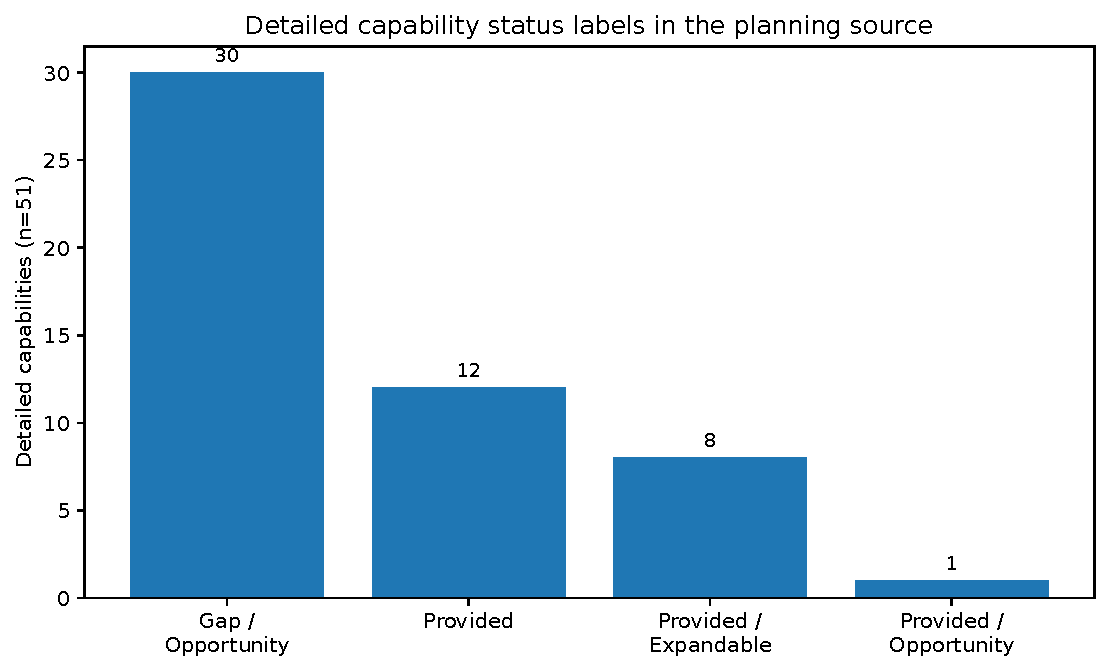
\includegraphics[width=.82\linewidth]{figures/fig1_status_composition.pdf}
\caption{Source-authored detailed capability labels. Gap/Opportunity is a planning label, not an observed service failure.}
\label{fig:status}
\end{figure}

\subsection{The scorecard does not independently reproduce the top priority without a decision rule}
The five score vectors are shown in Table~\ref{tab:score}. Equal weights give means of 4.6 (Firewall), 4.4 (IAM/PAM), 4.0 (DSPM), and 3.8 each (Human Risk and GRC). However, equal weighting is undocumented.

\begin{table}[H]
\centering
\small
\caption{Draft-3 focus-area score vectors and weight robustness. Criteria order is strategic fit, market demand, NOC readiness, SOC readiness, financial attractiveness.}
\label{tab:score}
\begin{tabularx}{\linewidth}{X c c X}
\toprule
Focus area & Score vector & Equal-weight mean & Relation to Firewall under arbitrary nonnegative normalized weights \\
\midrule
Managed Firewall Services & (5,4,5,4,5) & 4.6 & Reference \\
Managed IAM \& PAM & (5,4,4,4,5) & 4.4 & Firewall weakly dominates \\
Managed GRC & (4,3,4,3,5) & 3.8 & Firewall weakly dominates \\
DSPM / Data Privacy & (4,4,3,5,4) & 4.0 & Weight-sensitive \\
Human Risk / AI Awareness & (3,5,3,4,4) & 3.8 & Weight-sensitive \\
\bottomrule
\end{tabularx}
\end{table}

For DSPM,
\[
\mathrm{Firewall}\ge\mathrm{DSPM}
\iff
w_{\mathrm{strategic}}+2w_{\mathrm{NOC}}+w_{\mathrm{financial}}
\ge w_{\mathrm{SOC}}.
\]
For Human Risk,
\[
\mathrm{Firewall}\ge\mathrm{Human}
\iff
2w_{\mathrm{strategic}}+2w_{\mathrm{NOC}}+w_{\mathrm{financial}}
\ge w_{\mathrm{demand}}.
\]
Putting all weight on SOC readiness makes DSPM score 5 versus Firewall 4; putting all weight on market demand makes Human Risk 5 versus Firewall 4. Thus the numeric scorecard alone does not identify a unique top alternative. This is established MCDA sensitivity \cite{Maliene2018}. The final narrative nevertheless explicitly selects Firewall as the Year-1 flagship based on delivery fit and NOC readiness; our result is therefore a reproducibility boundary for the \emph{scorecard}, not a claim that the management choice is invalid.


\paragraph{Positive-weight robustness and decision boundary.}
The score vector for Firewall is $(5,4,5,4,5)$; its nonnegative differences against IAM/PAM and GRC establish \emph{weak} pairwise preference over both under every nonnegative normalized diagnostic weight vector. At corner weights, ties remain possible; this does not make Firewall a necessary \emph{unique} overall leader. The DSPM and Human Risk differences each include one negative coordinate, so that pairwise certificate fails. The strict-positive examples in Table~\ref{tab:positive-weights} establish alternative \emph{unique} winners without assigning zero weight to any criterion. These vectors are transparently chosen counterexamples, not observed preferences or a sample from a presumed weight distribution.
\begin{table}[H]
\centering\footnotesize
\caption{Strictly positive illustrative numerical weights; values are direct arithmetic on the source scores, not an elicited company rule.}
\label{tab:positive-weights}
\begin{tabularx}{\linewidth}{>{\raggedright\arraybackslash}p{4.0cm} r r X}
\toprule
$(w_S,w_D,w_{NOC},w_{SOC},w_F)$ & Firewall & Alternative top score & Top alternative\\
\midrule
$(0.10,0.20,0.10,0.50,0.10)$ & 4.30 & 4.40 & DSPM / Data Privacy\\
$(0.10,0.60,0.05,0.10,0.15)$ & 4.30 & 4.45 & Human Risk / AI Awareness\\
\bottomrule
\end{tabularx}
\end{table}
These findings distinguish (a) a robust \emph{pairwise} dominance certificate, (b) a nonunique \emph{global} top-ranked focus across an explicitly hypothetical weight class, and (c) the company's separately documented narrative proposal to launch Firewall first. The numeric score vectors were labelled ordinal in the source; interpreting them as cardinal additive contributions is itself an analysis-only assumption. Consequently these cases cannot identify the company's actual managerial preference or disprove the narrative choice.


\subsection{One direct stage conflict and five broader maturity signals}
The detailed capability years are 24/17/10 for Years 1/2/3, while package labels are 12/8/5. Exactly one mapped capability is later than its package: Control Effectiveness Monitoring is Year 2 inside a combined Year-1 GRC package. Under the strict all-components-at-launch convention, only this package moves, producing 11/9/5 (Figure~\ref{fig:stage}; Appendix~\ref{app:stage}).

The roadmap also names advanced scope later for five packages (S08, S21, S22, S24, S25), including NGWAF, SASE/lifecycle, OT/ICS, OT/IoT SOC, and microsegmentation. A broader sensitivity that treats each later-named milestone as first full-scope eligibility gives 7/11/7. That is not an approved schedule. Both an early limited-scope launch and a later full-scope maturity interpretation remain compatible with the source unless the service tier and acceptance scope are explicitly versioned.

\begin{figure}[H]
\centering
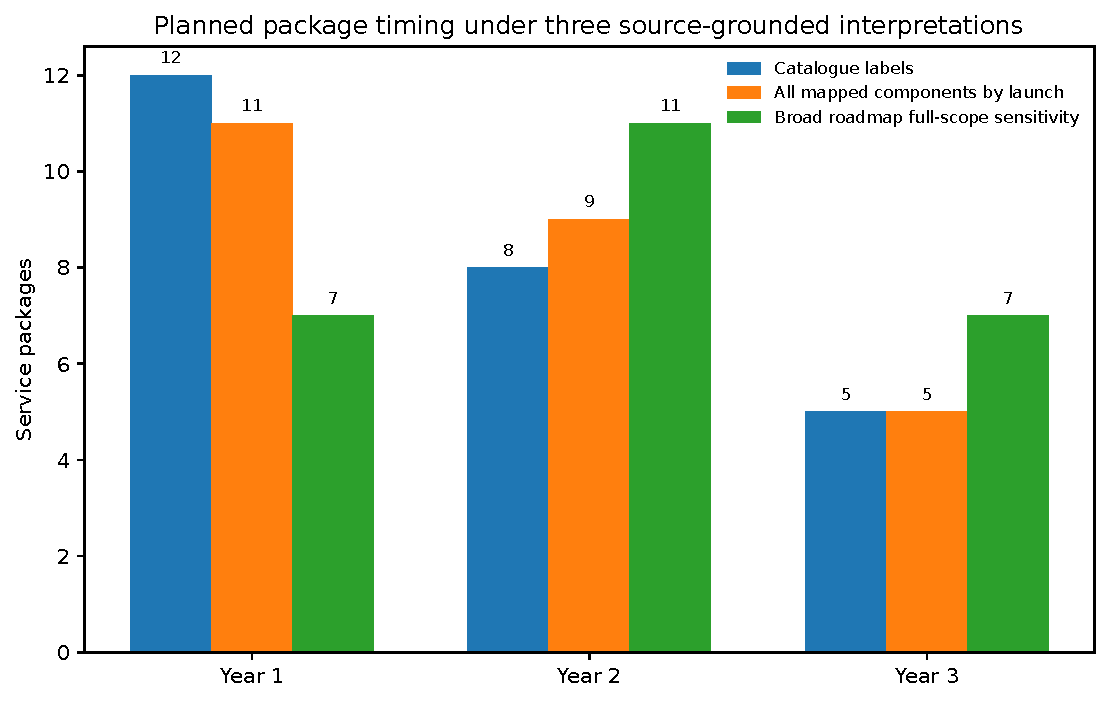
\includegraphics[width=.82\linewidth]{figures/fig2_stage_sensitivity.pdf}
\caption{Nominal package years and two explicit sensitivities. Neither sensitivity is an observed deployment schedule.}
\label{fig:stage}
\end{figure}

\subsection{Service-level financial effects are structurally underidentified}
The final scenario reports a normalized three-year revenue index of 1.000 across five service families. The amount itself is scenario-conditioned: because no country-level revenue split exists, the workbook applies an editable 12\% allocation for an excluded market, i.e., a 0.88 market factor.

No source record allocates family totals to the 25 packages or individual components. Under the favorable additive decomposition, Year 1 has 12 service-level unknowns and three independent family totals, Year 2 has 20 versus four, and Year 3 has 25 versus five. Across annual decompositions there are 57 unknowns but only 12 independent equations, leaving 45 free dimensions (Figure~\ref{fig:fin}).


The $45$ dimensions characterize an \emph{allocation vector}, not every target or comparison. Applying Section~\ref{sec:target-bounds} to a normalized family-year group gives the exact illustrative distinctions in Table~\ref{tab:financial-targets}; no company-specific per-package financial values or customer margins are inferred.
\begin{table}[H]
\centering\footnotesize
\caption{Exact bounds for target questions in a normalized group of total $Y=1$; mathematical illustrations, not observed company allocations.}
\label{tab:financial-targets}
\begin{tabularx}{\linewidth}{>{\raggedright\arraybackslash}p{4.0cm} c X}
\toprule
Target in a two-service group & Identified interval & Interpretation\\
\midrule
Family total $r_1+r_2$ & $[1,1]$ & Identified even though individual shares vary\\
One service $r_1$ & $[0,1]$ & Not identified without another legitimate restriction\\
Difference $r_1-r_2$ & $[-1,1]$ & Sign and implied preference are unresolved\\
Singleton-group service $r_1=Y$ & $[1,1]$ & Identified when the source group really has one member\\
\bottomrule
\end{tabularx}
\end{table}
The target-bound result is positive as well as negative: the family total is sufficient for a \emph{family-total question} even though it is insufficient for an individual service-revenue question. We do not equate a financial share with the commercial advantage of launching or delaying a service, which additionally depends on admissible costs, substitute sales, contracts and timing.


For any positive family-year total $Y$ with $k\ge2$ services, both the equal split $Y/k$ and a distinct positive allocation assigning $2Y/3$ to one service and $Y/[3(k-1)]$ to each other service reproduce the same aggregate. For example, in a separate normalized two-service illustration, $(0.5,0.5)$ and $(0.75,0.25)$ both sum to one. These are algebraic witnesses, not company service revenues. With one disjoint equation for each of the 12 positive family-year groups, the block-incidence matrix has rank 12; its 57 columns therefore leave a 45-dimensional nullspace. The assumptions and normalized witness are detailed in Appendix~\ref{app:finance-proof}. A package's revenue share is not identified, and a delay effect would additionally require marginal costs, customer retention and contract timing.

The workbook also encodes two post-resource conventions. Normalized by planned three-year revenue, the report-selected convention yields 0.3274 after resources, whereas the workbook's service-row convention yields 0.4109; the difference is 0.0835 of planned revenue. The discrepancy requires an owner-approved accounting definition; neither quantity is realized profit. A dashboard cell additionally contains \texttt{COUNTA(\#REF!)}.

\begin{figure}[H]
\centering
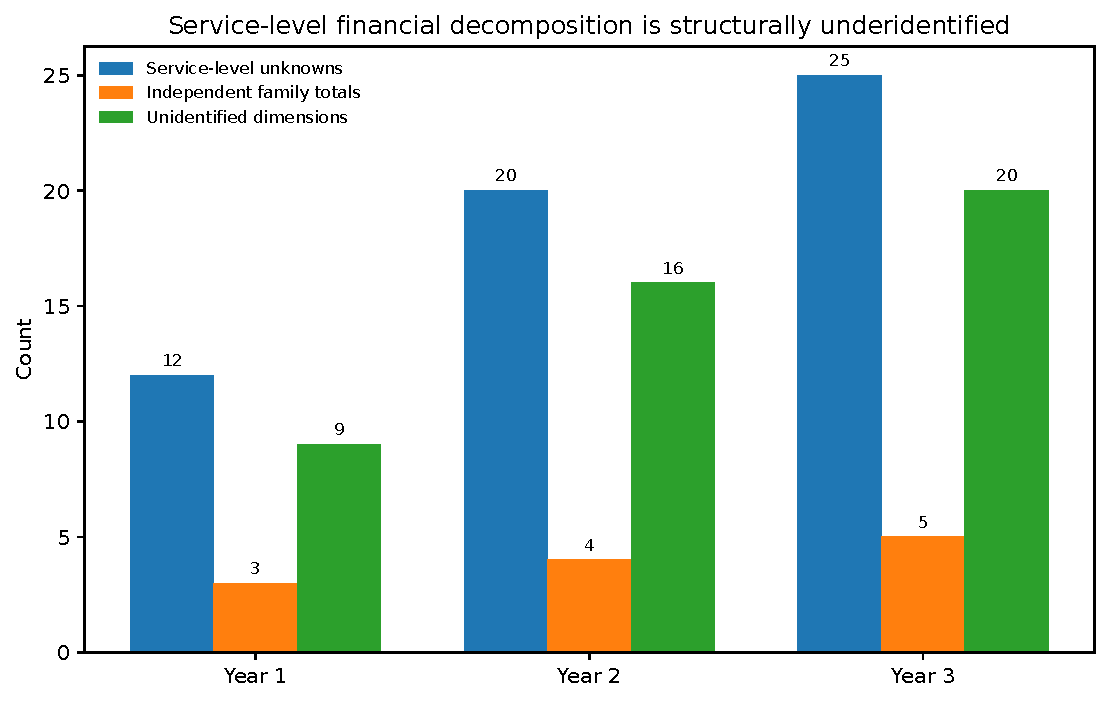
\includegraphics[width=.82\linewidth]{figures/fig3_identifiability.pdf}
\caption{Service-level financial decomposition is structurally underidentified even under a simple additive model favorable to identification.}
\label{fig:fin}
\end{figure}

\subsection{The source defines launch prerequisites but does not document their closure}
The plan itself warns against over-promising before delivery capability, tools, and NOC/SOC handoff are mature. Its Year-1 exit criteria require at least three lighthouse clients, a working SLA process, approved monthly reporting, and a tested firewall risk-score model. The 90-day plan calls for catalogue/pricing/RACI approval, runbooks/tooling, team preparation, and lighthouse pilots before external launch.

The supplied archive documents these as planned actions and targets (Appendix~\ref{app:release}). A separately hash-checked final-week reflection says the refined plan was presented to management for approval; no later approval minute is supplied. The archive does not contain a dated closure of the exit criteria, signed service-release acceptance, observed KPI numerators/denominators, or realized service-level revenue. Accordingly, the documentary disposition for achieved operational release is \textsc{Outcome evidence absent}; the number of packages actually released is unknown, rather than established as zero.

\section{Discussion}
\subsection{A roadmap can be coherent yet not decision-identifiable at the requested granularity}
The case does not show that the roadmap is wrong. It shows that different claims require different evidence granularity. Capability membership and final package labels are identified. Full-scope availability, the numerical scorecard's top alternative and service-level economics are not identified without additional rules; achieved operational readiness and KPI performance lack the required outcome observations in this archive.

The important distinction is between \emph{portfolio coherence} and \emph{claim identifiability}. The final mapping is complete, the planning narrative explicitly prefers Firewall, and the roadmap anticipates staged maturity; the supplied documents do not certify final management approval. Yet the same evidence does not uniquely answer every service-level counterfactual later asked of it.

\subsection{When incomplete evidence does and does not constrain a decision}
An optimization model may be well posed \emph{without} point identification of every input: robust choice can use an admitted uncertainty set and establish that a selected action remains justified over that set. The present archive has no documented service-level commercial utility or approved scorecard weight region with which to certify an actual deferral decision. In its absence, imposing an arbitrary share, score rule or launch interpretation would manufacture a managerially attributed conclusion. The target-level results above show why the prior question is not ``are all parameters known?'' but ``do the admissible facts and stated decision rule justify this \emph{particular} output?'' Missing acceptance records likewise provide no evidence of failure.

To implement the claim gate, each audit record declares (i) the requested claim and unit, (ii) source version/time/provenance, (iii) the constraints actually supported by each admitted artifact, (iv) a separately labelled assumption class if one is examined, (v) either a constant-answer value, target interval, robust-action witness, contradictory admitted same-scope assertions, or an absent-outcome reason, and (vi) an additional-evidence request with a stated authority and effective-scope requirement. The accompanying machine-readable casebook and tests demonstrate these outputs; they do not automate semantic judgment or make the protocol externally validated.

The proposed decision-specific audit sequence is therefore:
\begin{enumerate}[leftmargin=1.5em]
\item lock the source versions and distinguish explicit source assertions from analytic queries and unconfirmed intended uses;
\item validate source identity, unit, scope and capability/package traceability before joint admission;
\item preserve component semantics when testing aggregate claims;
\item declare which numerical rule class is only diagnostic; test weight sensitivity and robust pairwise preference separately;
\item distinguish nominal launch, minimum viable scope, and full-scope maturity;
\item test exact bounds of the requested financial target; do not equate an allocation with a delay counterfactual;
\item require observed release/assessment evidence before promoting planning states to operational readiness, and document what authorized record would permit a reassessment.
\end{enumerate}
This complements portfolio optimization, MCDA, repository integration, assurance cases, partial identification, OSCAL, and security measurement; it does not replace them. Compared with the six-company evidence-management interview study, this paper offers narrower executable, within-case decision witnesses rather than cross-organization findings. Compared with assurance-case defeater discovery, it checks algebraic uniqueness and admissible planning scope rather than constructing an assurance argument about system safety or security \cite{MohamadEvidence2024,Viger2026}. These case-specific witnesses are logically informative, but they do not constitute a randomized comparison of audit approaches. Each admitted test has a specific value, interval, conditional witness or missing-evidence reason, not a numerical ``quality score''. Unadmitted cross-unit assertions are recorded as an admission hold rather than artificially forced into a source conflict.

\subsection{Systems research comparators and the system boundary}
Recent systems-oriented studies offer particularly informative comparisons. Kocaoglu's purchasing-process roadmapping artifact uses differentiated capability profiles and explicit prioritization to link assessment to planned intervention, supported by expert development and multiple pilot applications \cite{Kocaoglu2026}. The present study does not introduce or externally validate a competing maturity instrument; it checks whether \emph{pre-existing} MSSP package and score records identify the decision at the requested granularity. Plevnik's security-sensitive information-systems service-governance case includes interviews and longitudinal incident data \cite{Plevnik2026}, providing operational evidence that our \emph{planning-only} archive lacks. Fowler et al.'s model-based cyber evaluation toolkit links system threats, proposed controls, and management decisions and includes practitioner face-validity evidence \cite{Fowler2024}; our test concerns source-to-portfolio decision admissibility, not threat-control effectiveness or expert-rated tool utility. Chen et al. distinguish digital traceability from verified evidence and physical compliance in a normative battery-identity governance model \cite{Chen2026}; our narrower counterpart is a deterministic documentary witness that traceable package and financial records can still leave a specified decision non-unique. Thus neither traceability insufficiency nor decision transparency is claimed as a new general principle.

The systems-level contribution here is a bounded account of how \emph{information loss, missing decision rules, inconsistent planning scopes, and absent outcome records} propagate across interdependent stages of one service-portfolio planning system. The claim gate locates the missing evidentiary link, and the target-level certificates also establish where a known family total or robust pairwise score comparison is already sufficient. The evidence-request register identifies records needed for reassessment, but does not prove a mathematically minimum evidence set. It is not a tested intervention, an operational assurance certification, a demonstrated productivity gain, or a multi-organization validation of a systems theory.

\subsection{Case-based contrast with an inventory-only check}
The case permits a narrow, reproducible ablation of \emph{questions}, not a comparison of auditor accuracy. A minimal document-presence check asks only whether a relevant record or label is present; it does not claim to establish sufficiency. Table~\ref{tab:contrast} shows what the claim-typed protocol additionally resolves when the intended question is made explicit. The examples and comparator were defined from the fixed source set, and no independent expert ground truth, time saving or false-reassurance rate is claimed. Assurance cases and OSCAL already handle claims and supporting evidence; this contrast does not demonstrate superiority over those richer methods \cite{Mohamad2021,OSCALAR2026,OSCALMapping2026}.
\begin{table}[H]
\centering\footnotesize
\caption{Document presence versus an identified decision claim: source-grounded examples, not an auditor-performance benchmark.}
\label{tab:contrast}
\begin{tabularx}{\linewidth}{>{\raggedright\arraybackslash}p{2.55cm} >{\raggedright\arraybackslash}p{3.15cm} X}
\toprule
Question & Document-presence observation & Additional claim-gate finding \\
\midrule
51 detailed capabilities? & Catalogue and 49 helper/narrative present & 51 directly enumerable; cross-label equivalence held pending definition of ``service versus ``capability \\
Component-wise predicate from package label? & Provided/Expandable appears on S06 and S07 & Not identified from label: opposite strict predicates \\
Scorecard's unique top focus? & Five score vectors present & Not identified absent rule; three alternative weight vectors give different winners \\
Individual package revenue? & Family-year totals present & Not identified: 57 unknowns, rank 12 under stated additive model \\
Actual Year-1 release? & Launch plan and exit criteria present & Outcome evidence absent; neither operational success nor failure established \\
\bottomrule
\end{tabularx}
\end{table}

\subsection{Additional evidence required for reassessment}
A held claim can be revisited only when a relevant additional observation or decision rule has been admitted. Table~\ref{tab:minimum} lists candidate authorized records; it does not establish minimal cardinality, monetary cost, or irreducibility of an evidence set. Every record would still need version, scope, date and authority checks before the output changes.
\begin{table}[H]
\centering\footnotesize
\caption{Additional records required for reassessment of held questions; their existence, authority and formal minimality are unverified.}
\label{tab:minimum}
\begin{tabularx}{\linewidth}{>{\raggedright\arraybackslash}p{2.4cm} X X}
\toprule
Held decision & Additional owner-approved record / rule & What it could identify \\
\midrule
Numerical priority & Criteria meaning, aggregation rule, admissible weights, tie policy and signed decision record & Reproducible numeric ordering, distinguished from narrative choice \\
Package full-scope launch & Component and service-tier definitions, time-stamped release and acceptance gates & Specific scope ready at a specified date, not quality in all settings \\
Package delay economics & Per-package commercial allocation/tariff, customer/contract horizon, avoidable-versus-shared cost and displacement rule & Defined scenario effect on contribution, conditional on assumptions \\
KPI achievement & Period-level observed counts, denominators, scope, collection rule and QA record & Realized KPI for the reported period, not causal impact \\
Executive authorization & Signed approval/decision minutes and versioned launch-governance disposition & Approval of the named plan, not completed implementation \\
\bottomrule
\end{tabularx}
\end{table}


\subsection{Portable protocol, independent interpretation and evidence-repair gates}
The companion \emph{source-free} repository now includes a claim-origin register, an input/output schema, a stepwise evidence-admission specification, exact algebraic target-bound routines, and deterministic tests. These specify what another analyst would have to examine, but do not themselves check the authority of an organizational document. The separation between a pre-admission \textsc{hold}, a logical result, its value or interval, and the reason for missing operational evidence is crucial for implementers; these fields can be used without changing the underlying archived source values.

A genuinely independent application study remains \textsc{not executed}. It would require permission-cleared matched source excerpts and at least two analysts not involved in developing the casebook, with frozen claims, blind dispositions, adjudication records and transparent denominators for any agreement statistic. A post-snapshot \emph{evidence repair} also remains \textsc{not executed}: an actual authorized dated weight rule, service-tier acceptance record, or approved accounting policy would need to be acquired and independently admitted before rerunning the \emph{same} held question. Merely supplying illustrative weights, running more software unit tests or adding hypothetical finance allocations cannot be described as a validated repair. These are explicit future evaluation gates rather than results of this paper.


\subsection{Implications for MSSP governance}
Three governance implications follow, qualified by whether the intended managerial use has actually been documented. First, a commercial package label should not substitute for component evidence when the decision is component-sensitive. Second, scorecards should publish the aggregation rule and weight rationale if the numeric ranking is intended to justify a priority decision. Third, the financial model should preserve a documented bridge from family forecast to package price, customer denominator, shared staffing, and avoidable cost if package-level delay economics are to be claimed.

The case's NOC/SOC role matrix reinforces the point: responsibility, specialist accountability, service delivery, and customer approval can sit with different actors. A service can therefore be commercially defined before all evidence needed for operational acceptance exists.

\section{Limitations and Claim Boundaries}
This is a single prospective industrial planning case, not a statistical sample of MSSPs. There is no second-company replication or independent blind coding. A finite source-level witness supports the stated counterexample, not claims of improved audit accuracy or external predictive validity. The 25 archive entries include duplicates, alternative document representations and non-analytical context; they are not 25 independent observations. The 51 detailed capabilities likewise are not independent field replications. It does not observe deployments, customer outcomes, realized revenue, SLA performance, or incident effectiveness. The source-authored status vocabulary is not a universal maturity scale.

The weighted-sum scorecard analysis is diagnostic because the source does not specify that weighted summation was its intended aggregation rule. Its purpose is to prove that the raw score matrix alone is insufficient to reproduce a unique top choice, not to recommend alternative weights. The 11/9/5 and 7/11/7 stage schedules are sensitivities, not recommended launch plans. The additive financial decomposition is intentionally favorable to identification and is not claimed to describe billing practice. The 12\% excluded-market adjustment is an explicit planning assumption necessitated by missing country-level revenue splits.

The literature-lineage comparisons are conceptual and source-test linked, not direct replications or empirical head-to-head evaluations of existing portfolio, repository, or security-assurance approaches. In particular, any improvement over a trained auditor, an OSCAL implementation, or a full assurance-case review remains untested. The study confines capability-to-package matching to a source-integrity control, not an evaluation of managed-service obligations, role-level assurance, or security-control compliance; those require a distinct unit of analysis and should not be confused with these decision-identifiability results. Only the limited, de-identified derived-data and executable-code capsule specified in the Data Availability Statement has been released publicly; access to original organizational records remains restricted and requires separate data-owner permission. For this named-author manuscript, the industrial case remains de-identified and financial quantities are normalized; this does not imply double-blind peer review. The authors' role in creating the original organizational plan, the intended managerial use of the analyst-defined queries, and authorization to disclose the particular industrial case findings have not been independently established from the available public source record. The original authors and data owner must review case provenance, permission and possible competing interests before journal submission. The public tests establish deterministic behavior after evidence admission, not independent semantic agreement. 

The protocol has not yet been replicated on a second MSSP portfolio, so cross-company transferability remains a methodological proposition rather than an empirical estimate.

\section{Conclusion}
A cybersecurity service roadmap can be internally traceable while failing to identify every decision later asked of it. In this 25-service MSSP case, all 51 detailed capabilities map exactly once to the final packages, but a hard-coded 49-service summary conflicts with their enumeration, package labels compress component semantics, the numerical scorecard lacks a decision rule that uniquely determines the top alternative, one direct component/package timing conflict and several later maturity signals create scope ambiguity, and family-level finance cannot identify service-level economics. The source also specifies launch prerequisites without supplying evidence of their closure.

The practical lesson is \emph{claim-specific evidence sufficiency}: distinguish what sources say, what an analyst asks, and what a decision actually requires. In this case the complete 51-to-25 mapping and the known family-year totals can answer source-membership and whole-group questions, while aggregate package labels, the undocumented numerical score rule, full-scope launch claims and individual revenues require more qualified interpretations. Exact pairwise score dominance and aggregate financial target bounds also show that nonuniqueness of an input need not imply nonuniqueness of every target or action. These are conditional, reproducible documentary and mathematical certificates within one case, not field validation. Future independent human application and a genuine authorized evidence-repair test are necessary before stronger effectiveness or portability claims.



% MDPI required author and research statements: unresolved human declarations remain explicit.
\authorcontributions{\textbf{Author confirmation required before submission.} The project-specific CRediT roles for M.E. and G.M. have not yet been confirmed by the individual authors. Authorship order does not establish the division of conceptualization, analysis, validation, manuscript preparation, or supervision.}
\funding{\textbf{Author confirmation required before submission.} The presence or absence of research funding, grant support, institutional sponsorship, or article-processing-charge support has not been verified for this manuscript. No funding or no-funding declaration is inferred.}
\institutionalreview{Not applicable. The study audits archival planning documents and reports no research intervention involving human or animal participants.}
\informedconsent{Not applicable. No study participants were recruited.}
\dataavailability{A public source-free reproducibility capsule containing de-identified derived inputs, a claim-decision casebook, deterministic arithmetic and logic checks, software regression tests, and the author-review PDF is available at \url{https://github.com/shaikhamalkawi-ux/mssp-decision-evidence-audit}. The fixed source-free code and schema snapshot is identified by \href{https://github.com/shaikhamalkawi-ux/mssp-decision-evidence-audit/commit/14be6c6affa0ca163299f325067f7d2b9b42e78e}{GitHub commit \texttt{14be6c6affa0}}; it contains the target-bound/robust-preference routines and reproducibility-scope documentation. The capsule reproduces the selected derived witnesses and algorithmic semantics; its source-free target-bound extension and schema are documented separately. Neither the release nor its unit tests reproduce the full original-workbook-to-manuscript pipeline, settle ambiguous source semantics or provide independent operational validation. Original company spreadsheets, reports, absolute financial records, exact source-path ledgers, and owner-controlled original-source replay code remain confidential and are not distributed. Requests for restricted source access require separate approval of the data owner and cannot be guaranteed. A previously executed owner-side checker reproduced 72 selected source-linked assertions, but those original records and checker are not in the public capsule. See Appendices A--D for the evidence and scope boundaries. Public visibility does not establish a license to redistribute the underlying corporate materials.}
\acknowledgments{OpenAI ChatGPT (GPT-6) assisted with English-language editing, literature discovery support, LaTeX preparation, code scaffolding, and consistency-check workflows during manuscript preparation. Such assistance does not constitute independent domain-expert validation, a new empirical experiment, or authorship. The human authors retain responsibility for verifying the source evidence, citations, calculations, code, and publication statements. The wording of this disclosure is subject to both authors' final review.}
\conflictsofinterest{\textbf{Author confirmation required before submission.} Project-specific financial, employment, organizational, and other potentially competing interests have not yet been declared by both authors. A positive declaration or a verified no-conflict statement must replace this notice before submission.}
\appendixtitles{yes}
\appendixstart
% Integrated editorial appendix. See the main manuscript for claim boundaries.
% Tables retain the values and source IDs of the previous de-identified supplement.
\clearpage
\appendix
\renewcommand{\thetable}{\Alph{section}\arabic{table}}
\renewcommand{\theHtable}{appendix.\Alph{section}.\arabic{table}}
\begingroup
\small
\setlength{\parskip}{3pt}
\setlength{\emergencystretch}{1.8em}

\section{Source archive and version reconciliation}\label{app:source}
\setcounter{table}{0}

\subsection{Source selection and analytical identity}\label{app:source-register}
The parent archive was fixed by SHA-256 before analysis. All nine analytical source files matched the internal source manifest byte-for-byte. The register uses de-identified source IDs; full source names remain in the confidential audit ledger.

\small
\begin{longtable}{p{0.55cm} p{2.2cm} p{2.1cm} p{7.1cm}}
\caption{De-identified source register and analytical roles.}\label{tab:app-source-register}\\
\toprule
ID & Artifact type & SHA-256 prefix & Role / principal audit finding \\
\midrule
\endhead
S1 & Earlier planning workbook & 4baf84570a33 & Earlier 10-area planning universe, five-market scope, Year-3 ARR scenario; internal roadmap/dashboard staging differences. \\
S2 & Earlier executive deck & 8b389fb63029 & Version context, ten new areas, pilot logic and immediate actions. \\
S3 & Earlier strategy roadmap & 0ec1fe47ce83 & Earlier customer targets, revenue ranges, dependencies and explicit scenario caveats. \\
S4 & Final planning workbook & 5efdcb233ffe & Primary quantitative source: 51 capabilities, five focus score vectors, years/statuses, KPI targets, financial/resource formulas and helper logic. \\
S5 & Final executive deck & 6aa9b25b568a & Final five-focus portfolio, firewall-led launch, exit criteria and 90-day launch actions. \\
S6 & Final report & 7cfdc29145a9 & Final roadmap/financial narrative, strategic over-promising risk, selected post-resource convention and launch prerequisites. \\
S7 & Consolidated catalogue PDF & 37cfc76d6bbd & 25 packages, 12/8/5 planned years, aggregate statuses and stale 49-to-25 narrative. \\
S8 & Mapping PDF & 3e3b7fde7d79 & Mapping display; stale 49 narrative despite 51 exact raw names in mapped strings. \\
S9 & Consolidation workbook & 1c41612214d7 & Machine-readable 25 packages and mappings; 51/51 raw names once each plus three explanatory phrases. \\
S10 & Final-week reflection PDF & 654d5f457b & Context-only: plan presented to management for approval; not evidence of executive acceptance or service launch. \\
\bottomrule
\end{longtable}
\small

\paragraph{Entry-level admission.} The immutable parent archive contains 25 entries: 23 material entries and two exporter-error texts. Two pairs of material entries are byte-identical weekly-reflection copies, leaving 21 distinct material payloads. Nine distinct analytical spreadsheet/PDF sources (S1--S9) enter the numerical and cross-format tests; one distinct final-week reflection (S10) enters \emph{only} the approval-status contextual check. Eleven other distinct material payloads were excluded from the numerical analysis as alternate editable representations, weekly context/presentation material, or presentation photographs. These are not extra independent case observations. The restricted entry-level ledger records each of the 25 original paths, its SHA-256, its disposition, and duplicate-of links; no unselected source was silently treated as contradictory numerical evidence.

\paragraph{Approval-status boundary (S10).} The final-week reflection (byte-identity SHA-256 prefix \texttt{654d5f457b}) states that the refined plan was presented to management for approval. A duplicate copy of the same PDF is present in the archive. This supports a proposal/submission-to-management claim, not proof of final approval or actual first-year release. No approval minute or later implementation closure was admitted in the archive.


\subsection{Differences between planning versions}\label{app:versions}
The two versions differ in decision universe, market scope, and financial metric.

\begin{center}
\captionof{table}{Differences between the earlier and final planning versions.}\label{tab:app-version-diff}
\begin{tabularx}{\linewidth}{p{3.0cm} X X}
\toprule
Dimension & Earlier version & Final version \\
\midrule
Portfolio object & 10 new areas plus references to identity and firewall work & 5 final focus areas; 51 detailed capabilities consolidated to 25 packages \\
Financial scope & Five-market scope & Four-market financial scope \\
Headline quantity & Year-3 ARR scenarios & Cumulative three-year planning revenue \\
Roadmap use & Foundation/scale/lead planning & Final five-focus staged implementation \\
Interpretation & Earlier planning version & Final planning version; not a realized outcome \\
\bottomrule
\end{tabularx}
\end{center}

The earlier version also contains internal staging differences: Human Risk/AI appears in different years across its dashboard/catalogue and roadmap, and one Year-1 dashboard priority is omitted from the roadmap's Year-1 key-service cell. These are differences between planning versions, not observed delivery failures.


\subsection{Cross-format reconciliation controls}\label{app:cross-format}
Four final-plan features reconcile across the source representations: (1) the same five focus areas and staged Year-1/2/3 logic appear in the workbook, final report, and executive deck; (2) the consolidation workbook and the paired catalogue PDFs agree on 25 packages and the nominal 12/8/5 split; (3) the report-selected financial totals agree with the final excluded-market planning sheet under the selected convention; and (4) the eight KPI trajectories match between workbook and final report. These controls show that the audit isolates claim-specific boundary problems rather than treating every source difference as an error.


\subsection{The 49-versus-51 source discrepancy}\label{app:count-conflict}
Direct enumeration of the final workbook yields 51 capability rows with year counts 24/17/10. The helper block instead displays 49 total services and 21/18/10.

Relevant workbook mechanics:
\begin{itemize}[leftmargin=1.4em]
\item the total-services helper is hardcoded at 49;
\item a status helper uses \texttt{COUNTIF(E14:E199,"*Provided*")}, starting below the first two identity-service detail rows, both labelled Provided;
\item the displayed total helper points back to the hardcoded 49;
\item the 21/18/10 year helper values are not linked to the complete detailed-year enumeration.
\end{itemize}
These checks establish a non-exhaustive status-helper range and a hard-coded summary of 49. The range omission excludes two Provided-containing rows, but it does not establish the historical origin of the 49 summary, demonstrate an automatic link to the package PDFs, or explain every year-count difference.


\section{Capability aggregation, priorities, and stages}\label{app:aggregation}
\setcounter{table}{0}

\subsection{Mapping and component-status composition}\label{app:mapping-status}
The 25-package mapping contains 54 semicolon-delimited phrases: 51 exact matches to all 51 detailed capability names, each once, plus three explanatory phrases.

Detailed status counts are 30 Gap/Opportunity, 12 Provided, 8 Provided/Expandable, and 1 Provided/Opportunity. Across packages, 20/25 contain at least one Gap/Opportunity component; 11/25 contain only Gap/Opportunity components; 4/25 have every component in \{Provided, Provided/Expandable\}; and 1/25 has every component exactly Provided. These are documentary compositions, not measured maturity.


\subsection{Package-label information-loss witness}\label{app:package-witness}
Using the exact source-name join from the final detailed capabilities (source S4) to the consolidation mapping (source S9, mapping rows 10--11), two packages share the aggregate label Provided/Expandable:
\begin{center}
\captionof{table}{Component-status witness for equal aggregate package labels.}\label{tab:app-witness}
\begin{tabularx}{\linewidth}{p{1.2cm} X p{2.0cm}}
\toprule
Package ID & Source-authored detailed component statuses & $g_{\mathrm{strict}}$ \\
\midrule
S06 & Provided; Gap/Opportunity; Provided/Expandable & 0 \\
S07 & Provided; Provided/Expandable & 1 \\
\bottomrule
\end{tabularx}
\end{center}
No component status was inferred from the aggregate package label; the strict predicate is a researcher-defined analysis question, not a company-approved launch condition. The original source-join script is supplied only in the author-controlled archive; the de-identified vectors and deterministic derived check are in \texttt{evidence/package\_label\_witness\_v8.json} and \texttt{code/check\_casebook\_v8.py}. This establishes information loss for the declared strict predicate, not actual operational performance.


\subsection{Prioritization sensitivity}\label{app:score}
The final workbook supplies five score vectors on criteria ordered as strategic fit, market demand, NOC readiness, SOC readiness and financial attractiveness:
\[
\begin{aligned}
\text{IAM/PAM}&=(5,4,4,4,5),\\
\text{DSPM}&=(4,4,3,5,4),\\
\text{Human Risk}&=(3,5,3,4,4),\\
\text{GRC}&=(4,3,4,3,5),\\
\text{Firewall}&=(5,4,5,4,5).
\end{aligned}
\]
No criterion weights or aggregation rule are supplied. The hypothetical numerical interpretation is not an owner-approved use of an ordinal scale. Equal-weight means are 4.4, 4.0, 3.8, 3.8 and 4.6 respectively. Firewall weakly dominates IAM/PAM and GRC, but not DSPM or Human Risk.

For nonnegative weights normalized to sum to one:
\[
\text{Firewall}\ge\text{DSPM}
\iff w_S+2w_N+w_F\ge w_{SOC},
\]
\[
\text{Firewall}\ge\text{Human}
\iff 2w_S+2w_N+w_F\ge w_D.
\]
All weight on SOC readiness makes DSPM 5 versus Firewall 4; all weight on market demand makes Human Risk 5 versus Firewall 4. The score matrix alone therefore does not reproduce a unique top focus area. Nevertheless, Firewall weakly dominates IAM/PAM and GRC across all nonnegative normalized diagnostic weights, and strictly positive example weights can make DSPM or Human Risk the unique winner; see Table~\ref{tab:positive-weights}. The final narrative separately identifies Firewall as the Year-1 flagship.


\subsection{Stage-consistency diagnostics}\label{app:stage}
Detailed component-year counts are 24/17/10; final package years are 12/8/5. One direct component/package conflict is present. The mechanical all-components-at-launch convention yields 11/9/5.

Five packages contain later-named roadmap milestones. A broader ``later milestone = first full-scope eligibility'' sensitivity yields 7/11/7. This is not an approved schedule and may overstate the meaning of later maturity/expansion entries.


\section{Financial identification and release prerequisites}\label{app:financial}
\setcounter{table}{0}

\subsection{Financial equation counts and normalized reconciliation}\label{app:finance-overview}
\begin{center}
\captionof{table}{Conditional degrees of freedom in the additive family-year decomposition.}\label{tab:app-finance}
\begin{tabularx}{\linewidth}{>{\raggedright\arraybackslash}X r r r r}
\toprule
Year & Service-year unknowns & Family totals & Rank & Free dimensions \\
\midrule
1 & 12 & 3 & 3 & 9 \\
2 & 20 & 4 & 4 & 16 \\
3 & 25 & 5 & 5 & 20 \\
\midrule
Total annual decompositions & 57 & 12 & 12 & 45 \\
\bottomrule
\end{tabularx}
\end{center}

Normalize planned three-year revenue to 1.000. Annual shares are 0.1081, 0.2966 and 0.5953. The final model applies a 0.88 market factor because an excluded market is represented by an editable 12\% allocation in the absence of country-level revenue splits.

Gross margin before resources is 0.4930 of planned revenue and modeled resource cost is 0.1655. The report-selected post-resource convention yields 0.3274; the workbook's alternative service-row convention yields 0.4109. The difference is 0.0835 of planned revenue. Neither quantity is a realized profit observation.


\subsection{Rank deficiency and non-unique allocation witness}\label{app:finance-proof}
Under the declared additive model, let $n_{fy}\geq1$ count the service-year entries inside active family $f$ in year $y$. Stack the 57 unknown nonnegative entries into $\mathbf r$; the 12 source family-year totals are $\mathbf Y=A\mathbf r$ where $A$ has one disjoint indicator row per family-year group. Its rows have non-overlapping nonempty supports and are therefore linearly independent, so
\[
 \operatorname{rank}(A)=12,\quad \dim\ker(A)=57-12=45.
\]
The rank statement describes the full allocation vector, not every possible target. Entire family-year totals remain identified, while arbitrary package shares are not. The exact conditional bound formula is in Section~\ref{sec:target-bounds}. The rank statement assumes these are the only independent equations and there are no additional observed service tariffs, contractual restrictions or package allocation records. The nonnegative feasible set is not automatically a linear space; ``45 free dimensions'' refers to the rank-nullity structure and, for strictly positive allocations and positive totals, its local feasible dimension.

For a normalized, two-service illustrative family-year block, the positive vectors
\[
\mathbf r^{(1)}=(0.50,0.50),\qquad \mathbf r^{(2)}=(0.75,0.25)
\]
both produce $Y=1$ but disagree about the revenue of the first service. If an actual family-year contains more services, hold their positive allocations fixed and transfer a small amount between any two positive entries; the same equation still holds. These numbers are \emph{algebraic illustrations}, not disclosed or reconstructed company revenue. A service delay's net cash consequence remains a distinct, stronger estimand requiring customer, tariff, substitution, avoidable-cost and time assumptions. Details and checks are provided in the executable casebook.


\subsection{Claim-decision record and inventory-only contrast}\label{app:casebook}
The locked, de-identified casebook \texttt{evidence/claim\_decision\_casebook\_v8.json} contains machine-readable claim/unit, admission, status, witness and missing-record fields. A document-inventory check can establish that a label, vector, total or plan is present; it cannot, \emph{by itself}, answer every stronger claim. The fixed five-row contrast in Table~\ref{tab:contrast} is a logical scope contrast, not a measured superiority, benchmark precision, time saving or independent-validation result. The companion script checks typed evidence, the package counterexample, three scorecard alternatives, and the normalized financial witness. No proprietary original sheet enters the de-identified package.


\subsection{Source-defined release evidence requirements}\label{app:release}
The final roadmap's Year-1 exit criteria are:
\begin{enumerate}[leftmargin=1.4em]
\item at least three lighthouse clients;
\item SLA process working;
\item monthly reporting approved;
\item firewall risk-score model tested.
\end{enumerate}
The 90-day plan additionally requires catalogue/service-tier/RACI/pilot-scope approval, runbooks and integration work, training, and lighthouse pilots before external launch. The supplied planning archive contains these requirements but no recorded closure decision for them.


\section{Additional audit observations and verification limits}\label{app:reproducibility}
\setcounter{table}{0}

\subsection{Additional source-document observations}\label{app:minor-observations}
Preserved for audit completeness but not used as central claims:
\begin{itemize}[leftmargin=1.4em]
\item one executive-dashboard cell contains \texttt{COUNTA(\#REF!)};
\item dashboard client counts point to a legacy financial sheet while revenue/margin text points to the updated-scope sheet; numeric client totals coincide in the inspected version;
\item the final report contains a one-day cover/prepared-date discrepancy;
\item one report sentence labels an adjusted-revenue value as a reverse-calculated serviceable-market estimate, while the workbook computes it as adjusted revenue; no alternative market-size conclusion is drawn.
\end{itemize}


\subsection{Claim states and conflict handling}\label{app:claim-states}
The audit uses a typed claim-admission rule before checking uniqueness. Formally, $\mathcal I(E_q)=\varnothing$ implies \emph{source conflict}, not vacuous identification. For example, the source helper reports 49 services while direct row enumeration counts 51 capabilities: this is a source-count discordance, not necessarily a genuine same-scope logical contradiction. The exact meaning of the source labels requires owner-side reconciliation before the two records may be admitted as jointly asserting an identical quantity. A nonempty set that admits different weighted-sum winners or positive financial allocations yields a claim classified as \emph{not identified}. In contrast, recorded nominal package years and exact mapping are \emph{identified as source facts}, while missing SLA or launch-acceptance records are classified as \emph{outcome evidence absent}. After admission and a specified precedence rule, these four display dispositions are distinct for each typed claim; missing required observations are separately encoded as a reason and a pre-admission scope hold is not classified as a conflict, and the presence of a plan cannot be counted as an observation of implementation.

The executable derived-data examples are contained in \texttt{code/claim\_gate\_demo.py}, \texttt{code/verify\_anonymized.py}, and the independent casebook check \texttt{code/check\_casebook\_v8.py}. This is a derived-data audit, not a distribution of original corporate sheets.

A separate, source-free regression suite checks 26 deterministic software properties of the typed claim gate, including rejection of cross-version, cross-unit and cross-definition assertions, explicit handling of empty interpretation sets, missing component statuses, tied scores and distinct positive allocations with the same total. These tests verify the declared program semantics on already specified examples. They do not constitute independent validation on 26 companies, new source-data tests or a complete raw-workbook-to-manuscript replay.


\subsection{Boundaries of the findings}\label{app:boundaries}
The study does not treat presentation for approval as final executive authorization and does not assert that any package failed, that all packages operated, that Firewall should be replaced as the strategic priority, that equal weights are the intended scorecard method, that either timing sensitivity is a recommended schedule, or that either post-resource quantity is realized profit. The contribution is the boundary between claims supported by the planning record and claims requiring a decision rule or observed operational evidence.


\subsection{Bounded original-workbook source-to-result rerun}\label{app:original-rerun}
An owner-side checker was implemented separately from the earlier anonymized-derived-data tests and run directly against the immutable original archive. It imports the two relevant Draft-3 XLSX payloads using a spreadsheet parser, joins the raw detailed capability names to the source-authored package mapping, recomputes the declared component-stage predicate and focus-score arithmetic, and recomputes the relevant normalized family-year financial identities. No original corporate workbook is included in the de-identified package.

\begin{center}
\begin{minipage}{\linewidth}
\centering\small
\captionof{table}{Scope and outcome of the selected original-source verification.}\label{tab:app-source-rerun}
\begin{tabularx}{\linewidth}{>{\raggedright\arraybackslash}p{3.25cm} X}
\toprule
Original-source gate & Recomputed outcome / scope\\
\midrule
Source and membership & Parent archive identity and 25-entry composition; two Draft-3 workbook checksums; 51 unique capability names, 51 exact one-to-one links, 25 packages, three non-matching explanatory strings.\\
Stage and labels & Detail-year 24/17/10, package-year 12/8/5, one later component, and the 11/9/5 all-components sensitivity; opposite strict predicates for source-anonymized S06/S07 under an equal aggregate label.\\
Scorecard & Five source score vectors recomputed; equal, SOC-only and demand-only illustrative weights have three different leaders. No weights are represented as the company's adopted rule.\\
Finance & Annual family revenue and gross-margin arithmetic, modeled resource-cost reconciliation, both post-resource conventions, 57 active package-year unknowns versus 12 positive family-year aggregates, and the conditional 45-dimensional linear nullspace. Only normalized ratios are released.\\
Not included in this gate & The 7/11/7 broad full-scope interpretation, semantic review of every PDF passage, global absence of operational records, causal claims, expert validation or cross-company replication.\\
\bottomrule
\end{tabularx}
\end{minipage}
\end{center}

The author-controlled runner passed 72 mechanically specified checks, including individual revenue, gross-margin and resource-row recomputations; these are not 72 statistically independent case observations. This strengthens reproducibility of the selected mechanical findings, not the paper's external validity. The exact original archive remains restricted. Reproduction at other institutions depends on legitimate authorized access to the source files, which cannot be replaced by the public derived-data package.



\subsection{Target-specific certificates and claim-origin limitations}\label{app:v18-certificates}
The decision-sufficiency extension is an analytical audit of the same already published score vectors and of an explicitly abstract additive family-year model. It does not introduce new company results. For the full nonnegative weight simplex, Firewall's weak pairwise advantage over IAM/PAM and GRC follows from componentwise dominance; it is not a guaranteed unique global winner. Positive hypothetical weights produce the DSPM and Human Risk counterexamples given in Table~\ref{tab:positive-weights}. The published ordinal source scores are not certified cardinal utilities.\par
For disjoint nonnegative allocation groups of positive totals, the bounds in Section~\ref{sec:target-bounds} follow by selecting the smallest/largest coefficient within each simplex block. An intact group total has bounds $[Y_g,Y_g]$, whereas one component of a group containing at least two entries can range from $0$ to $Y_g$ without extra restrictions. The entire 57-component allocation is not identified by the 12 totals; a subset total may still be identified if its membership is a union of complete groups. These mathematical cases should not be read as contractual allocations, financial recommendations or actual earnings.\par
The V18 source-free public extension includes a structured record schema, explicit claim-origin/intended-use register, and executable finite examples. Protocol-human interpretation and real evidence-repair experiments have \emph{not} been conducted. Every claim origin, source scope, authorizing decision and sharing permission must be supported by source or person-specific evidence before publication as a real governance result.

\endgroup

\reftitle{References}

\begin{thebibliography}{99}
% Author-review bibliography line spacing; preserves the template 9 pt font.
\fontsize{9}{10.5}\selectfont
\bibitem{Kohlborn2009} T. Kohlborn, E. Fielt, A. Korthaus, and M. Rosemann, ``Towards a Service Portfolio Management Framework,'' \emph{ACIS 2009 Proceedings}, Paper 21, 2009.
\bibitem{Comerio2015} M. Comerio et al., ``Service portfolio management: A repository-based framework,'' \emph{Journal of Systems and Software}, vol. 104, pp. 112--125, 2015. doi:10.1016/j.jss.2015.01.055.
\bibitem{BatiniComerio2016} C. Batini and M. Comerio, ``A Methodology for the Integration of Service Repositories,'' \emph{Communications of the IBIMA}, vol. 2016, article 790219, 2016. doi:10.5171/2016.790219.
\bibitem{LinHsieh2011} F.-R. Lin and P.-S. Hsieh, ``A SAT View on New Service Development,'' \emph{Service Science}, vol. 3, no. 2, pp. 141--157, 2011. doi:10.1287/serv.3.2.141.
\bibitem{MenorRoth2008} L. J. Menor and A. V. Roth, ``New Service Development Competence and Performance: An Empirical Investigation in Retail Banking,'' \emph{Production and Operations Management}, vol. 17, no. 3, pp. 267--284, 2008. doi:10.3401/poms.1080.0034.
\bibitem{Liesio2008} J. Liesi\"o, P. Mild, and A. Salo, ``Robust portfolio modeling with incomplete cost information and project interdependencies,'' \emph{European Journal of Operational Research}, vol. 190, no. 3, pp. 679--695, 2008. doi:10.1016/j.ejor.2007.06.049.
\bibitem{Tavana2019} M. Tavana, G. Khosrojerdi, H. Mina, and A. Rahman, ``A hybrid mathematical programming model for optimal project portfolio selection using fuzzy inference system and analytic hierarchy process,'' \emph{Evaluation and Program Planning}, vol. 77, 101703, 2019. doi:10.1016/j.evalprogplan.2019.101703.
\bibitem{GuptaZhdanov2012} A. Gupta and D. Zhdanov, ``Growth and Sustainability of Managed Security Services Networks: An Economic Perspective,'' \emph{MIS Quarterly}, vol. 36, no. 4, pp. 1109--1130, 2012.
\bibitem{Wu2017} D. Wu et al., ``Decision making in information security outsourcing: Impact of complementary and substitutable firms,'' \emph{Computers \& Industrial Engineering}, vol. 110, pp. 1--12, 2017. doi:10.1016/j.cie.2017.05.018.
\bibitem{Maliene2018} V. Maliene, R. Dixon-Gough, and N. Malys, ``Dispersion of relative importance values contributes to the ranking uncertainty: Sensitivity analysis of Multiple Criteria Decision-Making methods,'' \emph{Applied Soft Computing}, vol. 67, pp. 286--298, 2018. doi:10.1016/j.asoc.2018.03.003.
\bibitem{Cezar2017} A. Cezar, H. Cavusoglu, and S. Raghunathan, ``Sourcing Information Security Operations: The Role of Risk Interdependency and Competitive Externality in Outsourcing Decisions,'' \emph{Production and Operations Management}, vol. 26, no. 5, pp. 860--879, 2017. doi:10.1111/poms.12681.
\bibitem{Powell2008} S. G. Powell, K. R. Baker, and B. Lawson, ``A critical review of the literature on spreadsheet errors,'' \emph{Decision Support Systems}, vol. 46, no. 1, pp. 128--138, 2008. doi:10.1016/j.dss.2008.06.001.
\bibitem{Poon2024} P.-L. Poon, M. F. Lau, Y. T. Yu, and S.-F. Tang, ``Spreadsheet quality assurance: a literature review,'' \emph{Frontiers of Computer Science}, vol. 18, article 182203, 2024. doi:10.1007/s11704-023-2384-6.
\bibitem{Dawson2026} N. Dawson, E. Knight, I. Bongiovanni, and R. O'Quinn, ``Informed cybersecurity decisions: A synthesis of expert perspectives,'' \emph{Computers \& Security}, vol. 167, article 104927, 2026. doi:10.1016/j.cose.2026.104927.
\bibitem{GSNv3} Assurance Case Working Group, \emph{Goal Structuring Notation Community Standard}, Version 3, Safety-Critical Systems Club, 2021. \url{https://scsc.uk/resources/citation_r1386.html}.
\bibitem{SACM2023} Object Management Group, \emph{Structured Assurance Case Metamodel}, Version 2.3, October 2023. \url{https://www.omg.org/spec/SACM/2.3}.
\bibitem{Mohamad2021} M. Mohamad, J.-P. Stegh\"ofer, and R. Scandariato, ``Security assurance cases---state of the art of an emerging approach,'' \emph{Empirical Software Engineering}, vol. 26, article 70, 2021. doi:10.1007/s10664-021-09971-7.
\bibitem{MohamadEvidence2024} M. Mohamad, J.-P. Stegh\"ofer, E. Knauss, and R. Scandariato, ``Managing security evidence in safety-critical organizations,'' \emph{Journal of Systems and Software}, vol. 214, article 112082, 2024. doi:10.1016/j.jss.2024.112082.
\bibitem{Viger2026} T. Viger et al., ``Assessing the Usefulness of Assurance Cases: Experience With the Large Hadron Collider,'' \emph{Systems Engineering}, vol. 29, no. 1, pp. 99--113, 2026. doi:10.1002/sys.70010.
\bibitem{Manski2005} C. F. Manski, ``Partial identification with missing data: Concepts and findings,'' \emph{International Journal of Approximate Reasoning}, vol. 39, no. 2--3, pp. 151--165, 2005. doi:10.1016/j.ijar.2004.10.006.
\bibitem{OSCALMapping2026} National Institute of Standards and Technology, ``OSCAL Control Mapping Model,'' OSCAL Control Layer, accessed November 2026. \url{https://pages.nist.gov/OSCAL/learn/concepts/layer/control/mapping/}.
\bibitem{OSCALAR2026} National Institute of Standards and Technology, ``OSCAL Assessment Results Model,'' OSCAL Assessment Layer, accessed 2026.
\bibitem{OSCAL2026} National Institute of Standards and Technology, ``OSCAL System Security Plan Model v1.2.3: implementation-status,'' OSCAL Reference, accessed 2026.
\bibitem{NIST80055v1} K. Schroeder, H. Trinh, and V. Pillitteri, \emph{Measurement Guide for Information Security, Vol. 1: Identifying and Selecting Measures}, NIST SP 800-55 Vol. 1, 2024. doi:10.6028/NIST.SP.800-55v1.
\bibitem{NIST80055v2} K. Schroeder, H. Trinh, and V. Pillitteri, \emph{Measurement Guide for Information Security, Vol. 2: Developing an Information Security Measurement Program}, NIST SP 800-55 Vol. 2, 2024. doi:10.6028/NIST.SP.800-55v2.
\bibitem{NIST8477} K. Scarfone, M. Souppaya, and M. Fagan, \emph{Mapping Relationships Between Documentary Standards, Regulations, Frameworks, and Guidelines}, NIST IR 8477, 2024. doi:10.6028/NIST.IR.8477.
\bibitem{NIST1347} S. Quinn, D. Eliot, G. Witte, and B. Hoehn, \emph{NIST Cybersecurity Framework 2.0: Informative References Quick-Start Guide}, NIST SP 1347, August 2026. doi:10.6028/NIST.SP.1347.
\bibitem{Kocaoglu2026} B. Kocaoglu, ``A Process-Level Digital Maturity and Roadmapping Artifact for Purchasing: Development and Utility Demonstration of DEMA,'' \emph{Systems}, vol. 14, no. 5, article 532, 2026. doi:10.3390/systems14050532.
\bibitem{Plevnik2026} M. Plevnik, ``Communication and Information Systems User Support as a Governance Mechanism in a High-Security Public Organization,'' \emph{Systems}, vol. 14, no. 3, article 288, 2026. doi:10.3390/systems14030288.
\bibitem{Fowler2024} S. Fowler, K. Joiner, and S. Ma, ``Cyber Evaluation and Management Toolkit (CEMT): Face Validity of Model-Based Cybersecurity Decision Making,'' \emph{Systems}, vol. 12, no. 7, article 238, 2024. doi:10.3390/systems12070238.
\bibitem{Chen2026} Y. Chen, X. Liang, X. Xu, and C. Cao, ``From Traceability to Closed-Loop Accountability: A Stackelberg Model of Evidence Quality and Recycling Compliance for Emerging Electric-Vehicle Battery Digital Identity Governance,'' \emph{Systems}, vol. 14, no. 9, article 1038, 2026. doi:10.3390/systems14091038.
\end{thebibliography}
% Publisher boilerplate is inserted by MDPI at typesetting; omit in author-review PDF to avoid an orphan disclaimer page.
\end{document}
